% Copyright (C) 2026: The University of Edinburgh, United Kingdom
%                 Authors: Craig Warren, Antonis Giannopoulos, John Hartley,
%                          and Nathan Mannall
%
% This file is part of gprMax.
%
% gprMax is free software: you can redistribute it and/or modify
% it under the terms of the GNU General Public License as published by
% the Free Software Foundation, either version 3 of the License, or
% (at your option) any later version.
%
% gprMax is distributed in the hope that it will be useful,
% but WITHOUT ANY WARRANTY; without even the implied warranty of
% MERCHANTABILITY or FITNESS FOR A PARTICULAR PURPOSE. See the
% GNU General Public License for more details.
%
% You should have received a copy of the GNU General Public License
% along with gprMax. If not, see <http://www.gnu.org/licenses/>.
%
% The input TikZ file is the canonical editable source for both the LaTeX
% figure and images_shared/yeecell2dTEz.png. Compile this wrapper and rasterise
% its single PDF page to regenerate the documentation image. Convert the PDF
% with `dvisvgm --pdf --no-fonts` before rasterising: converting glyphs to
% paths prevents PDF importers from substituting the embedded TeX fonts.

\documentclass[tikz,border=4pt]{standalone}

\begin{document}
% Copyright (C) 2026: The University of Edinburgh, United Kingdom
%                 Authors: Craig Warren, Antonis Giannopoulos, John Hartley,
%                          and Nathan Mannall
%
% This file is part of gprMax.
%
% gprMax is free software: you can redistribute it and/or modify
% it under the terms of the GNU General Public License as published by
% the Free Software Foundation, either version 3 of the License, or
% (at your option) any later version.
%
% gprMax is distributed in the hope that it will be useful,
% but WITHOUT ANY WARRANTY; without even the implied warranty of
% MERCHANTABILITY or FITNESS FOR A PARTICULAR PURPOSE. See the
% GNU General Public License for more details.
%
% You should have received a copy of the GNU General Public License
% along with gprMax. If not, see <http://www.gnu.org/licenses/>.
%
% Input-ready TikZ source for the two-cell gprMax 2D TEz Yee-grid figure.
% The only required package is \usepackage{tikz}.

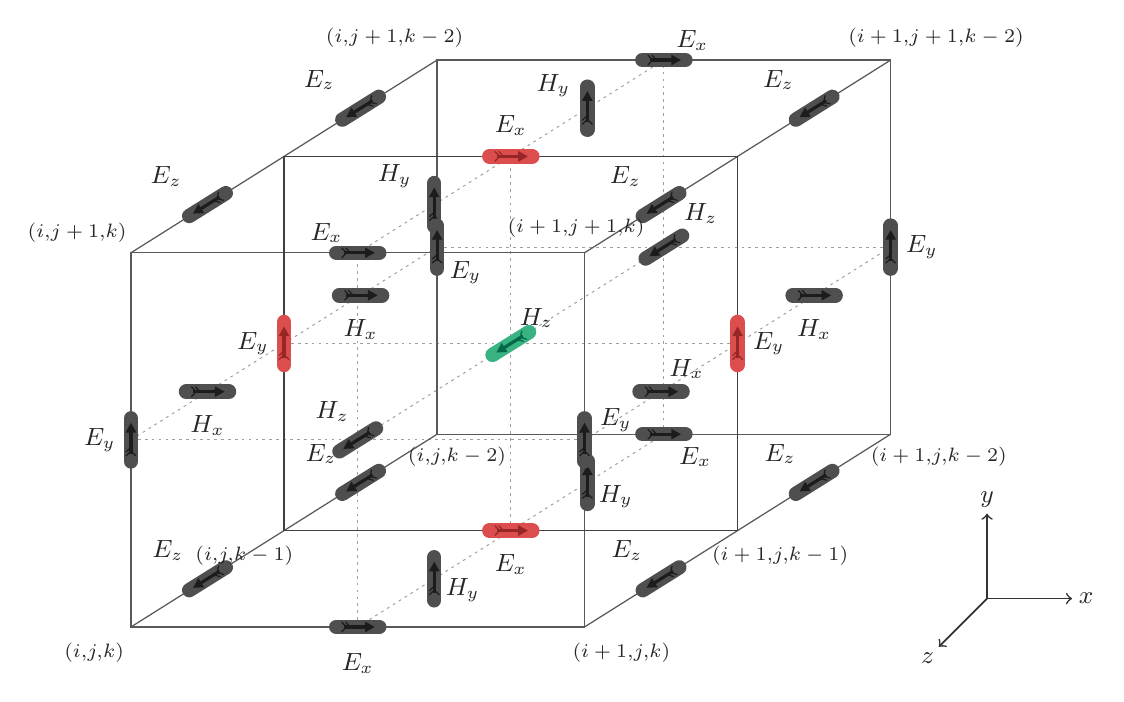
\begin{tikzpicture}[
    x=0.72cm,
    y=0.72cm,
    cell edge/.style={draw=black!65, line width=0.45pt},
    interior plane/.style={draw=black!75, line width=0.65pt},
    construction/.style={draw=black!38, line width=0.35pt, dash pattern=on 1pt off 1.5pt},
    field label/.style={font=\small\bfseries, text=black!85, inner sep=0pt},
    index label/.style={font=\scriptsize\bfseries\itshape, text=black!85, inner sep=0pt},
    axis label/.style={font=\small, text=black!85, inner sep=1pt}
]

% Colours deliberately match the PNG/SVG artwork.
\definecolor{yeeRed}{RGB}{220,78,78}
\definecolor{yeeRedDark}{RGB}{151,38,38}
\definecolor{yeeGreen}{RGB}{57,179,130}
\definecolor{yeeGreenDark}{RGB}{5,105,72}
\definecolor{yeeGrey}{RGB}{79,79,79}
\definecolor{yeeGreyDark}{RGB}{28,28,28}

% Compact rounded field vector centred at #1 and rotated by #2 degrees. #3 is
% the capsule colour and #4 is the arrow colour. The capsule is deliberately
% shadow-free so its centre remains visually coincident with the Yee location.
\newcommand{\yeeField}[4]{%
  \begin{scope}[shift={#1}, rotate=#2]
    \draw[draw=#3, line width=5.2pt, line cap=round]
      (-0.38,0) -- (0.38,0);
    \fill[#4] (-0.25,-0.028) rectangle (0.15,0.028);
    \fill[#4] (0.30,0) -- (0.13,0.095) -- (0.13,-0.095) -- cycle;
    \draw[draw=#4, line width=0.45pt, line cap=round, line join=round]
      (-0.28,0.085) -- (-0.20,0) -- (-0.28,-0.085)
      (-0.21,0.085) -- (-0.13,0);
  \end{scope}%
}

% Three x-y grid planes bound two cells in the invariant z direction:
% front k, shared interior k-1, and back k-2.
\coordinate (Fbl) at (0,0);
\coordinate (Fbr) at (8,0);
\coordinate (Ftl) at (0,6.6);
\coordinate (Ftr) at (8,6.6);
\coordinate (Mbl) at (2.7,1.7);
\coordinate (Mbr) at (10.7,1.7);
\coordinate (Mtl) at (2.7,8.3);
\coordinate (Mtr) at (10.7,8.3);
\coordinate (Bbl) at (5.4,3.4);
\coordinate (Bbr) at (13.4,3.4);
\coordinate (Btl) at (5.4,10.0);
\coordinate (Btr) at (13.4,10.0);

% Exact centres of the four x-z faces that carry the suppressed Hy fields.
% Defining these from face diagonals avoids any apparent/manual offset.
\path (Fbl) -- coordinate[midway] (HyFrontBottom) (Mbr);
\path (Ftl) -- coordinate[midway] (HyFrontTop) (Mtr);
\path (Mbl) -- coordinate[midway] (HyBackBottom) (Bbr);
\path (Mtl) -- coordinate[midway] (HyBackTop) (Btr);

% Cell-centre construction lines.
\begin{scope}[construction]
  \draw (4,0) -- (4,6.6) (0,3.3) -- (8,3.3);
  \draw (6.7,1.7) -- (6.7,8.3) (2.7,5) -- (10.7,5);
  \draw (9.4,3.4) -- (9.4,10) (5.4,6.7) -- (13.4,6.7);
  \draw (0,3.3) -- (2.7,5) -- (5.4,6.7);
  \draw (8,3.3) -- (10.7,5) -- (13.4,6.7);
  \draw (4,6.6) -- (6.7,8.3) -- (9.4,10);
  \draw (4,0) -- (6.7,1.7) -- (9.4,3.4);
  \draw (4,3.3) -- (6.7,5) -- (9.4,6.7);
\end{scope}

% Cell outlines and the shared interior plane.
\draw[cell edge] (Fbl) -- (Fbr) -- (Ftr) -- (Ftl) -- cycle;
\draw[cell edge] (Bbl) -- (Bbr) -- (Btr) -- (Btl) -- cycle;
\draw[cell edge] (Fbl) -- (Mbl) -- (Bbl);
\draw[cell edge] (Fbr) -- (Mbr) -- (Bbr);
\draw[cell edge] (Ftl) -- (Mtl) -- (Btl);
\draw[cell edge] (Ftr) -- (Mtr) -- (Btr);
\draw[interior plane] (Mbl) -- (Mbr) -- (Mtr) -- (Mtl) -- cycle;

% Suppressed Ez components on the z-directed edges of both cells.
\yeeField{(1.35,0.85)}{-148}{yeeGrey}{yeeGreyDark}
\yeeField{(9.35,0.85)}{-148}{yeeGrey}{yeeGreyDark}
\yeeField{(1.35,7.45)}{-148}{yeeGrey}{yeeGreyDark}
\yeeField{(9.35,7.45)}{-148}{yeeGrey}{yeeGreyDark}
\yeeField{(4.05,2.55)}{-148}{yeeGrey}{yeeGreyDark}
\yeeField{(12.05,2.55)}{-148}{yeeGrey}{yeeGreyDark}
\yeeField{(4.05,9.15)}{-148}{yeeGrey}{yeeGreyDark}
\yeeField{(12.05,9.15)}{-148}{yeeGrey}{yeeGreyDark}

% Suppressed Hx components at the centres of y-z faces.
\yeeField{(1.35,4.15)}{0}{yeeGrey}{yeeGreyDark}
\yeeField{(9.35,4.15)}{0}{yeeGrey}{yeeGreyDark}
\yeeField{(4.05,5.85)}{0}{yeeGrey}{yeeGreyDark}
\yeeField{(12.05,5.85)}{0}{yeeGrey}{yeeGreyDark}

% Suppressed Hy components at the centres of x-z faces.
\yeeField{(HyFrontBottom)}{90}{yeeGrey}{yeeGreyDark}
\yeeField{(HyFrontTop)}{90}{yeeGrey}{yeeGreyDark}
\yeeField{(HyBackBottom)}{90}{yeeGrey}{yeeGreyDark}
\yeeField{(HyBackTop)}{90}{yeeGrey}{yeeGreyDark}

% Inactive Ex, Ey, and Hz fields on the two outer PEC/PMC boundary planes.
\yeeField{(4,0)}{0}{yeeGrey}{yeeGreyDark}
\yeeField{(4,6.6)}{0}{yeeGrey}{yeeGreyDark}
\yeeField{(0,3.3)}{90}{yeeGrey}{yeeGreyDark}
\yeeField{(8,3.3)}{90}{yeeGrey}{yeeGreyDark}
\yeeField{(4,3.3)}{-148}{yeeGrey}{yeeGreyDark}
\yeeField{(9.4,3.4)}{0}{yeeGrey}{yeeGreyDark}
\yeeField{(9.4,10)}{0}{yeeGrey}{yeeGreyDark}
\yeeField{(5.4,6.7)}{90}{yeeGrey}{yeeGreyDark}
\yeeField{(13.4,6.7)}{90}{yeeGrey}{yeeGreyDark}
\yeeField{(9.4,6.7)}{-148}{yeeGrey}{yeeGreyDark}

% Active TEz fields on the shared interior plane.
\yeeField{(6.7,1.7)}{0}{yeeRed}{yeeRedDark}
\yeeField{(6.7,8.3)}{0}{yeeRed}{yeeRedDark}
\yeeField{(2.7,5)}{90}{yeeRed}{yeeRedDark}
\yeeField{(10.7,5)}{90}{yeeRed}{yeeRedDark}
\yeeField{(6.7,5)}{-148}{yeeGreen}{yeeGreenDark}

% Field labels: suppressed Ez.
\node[field label] at (0.65,1.35) {$E_z$};
\node[field label] at (8.75,1.35) {$E_z$};
\node[field label] at (0.62,7.95) {$E_z$};
\node[field label] at (8.72,7.95) {$E_z$};
\node[field label] at (3.35,3.05) {$E_z$};
\node[field label] at (11.45,3.05) {$E_z$};
\node[field label] at (3.32,9.65) {$E_z$};
\node[field label] at (11.42,9.65) {$E_z$};

% Field labels: suppressed Hx and Hy.
\node[field label] at (1.35,3.55) {$H_x$};
\node[field label] at (9.80,4.55) {$H_x$};
\node[field label] at (4.05,5.25) {$H_x$};
\node[field label] at (12.05,5.25) {$H_x$};
\node[field label] at (5.85,0.65) {$H_y$};
\node[field label] at (4.65,7.95) {$H_y$};
\node[field label] at (8.55,2.30) {$H_y$};
\node[field label] at (7.45,9.55) {$H_y$};

% Field labels: inactive outer-boundary Ex, Ey, and Hz.
\node[field label] at (4,-0.65) {$E_x$};
\node[field label] at (3.45,6.95) {$E_x$};
\node[field label] at (-0.55,3.3) {$E_y$};
\node[field label] at (8.55,3.65) {$E_y$};
\node[field label] at (3.55,3.80) {$H_z$};
\node[field label] at (9.95,3.0) {$E_x$};
\node[field label] at (9.9,10.35) {$E_x$};
\node[field label] at (5.9,6.25) {$E_y$};
\node[field label] at (13.95,6.7) {$E_y$};
\node[field label] at (10.05,7.30) {$H_z$};

% Field labels: active Ex, Ey, and Hz.
\node[field label] at (6.7,1.1) {$E_x$};
\node[field label] at (6.7,8.85) {$E_x$};
\node[field label] at (2.15,5) {$E_y$};
\node[field label] at (11.25,5) {$E_y$};
\node[field label] at (7.15,5.45) {$H_z$};

% Selected Yee indices make the two z cells explicit without over-labelling.
\node[index label] at (-0.65,-0.45) {$(i,\!j,\!k)$};
\node[index label] at (8.65,-0.45) {$(i+1,\!j,\!k)$};
\node[index label] at (-0.95,6.95) {$(i,\!j+1,\!k)$};
\node[index label] at (7.85,7.05) {$(i+1,\!j+1,\!k)$};
\node[index label] at (2.0,1.25) {$(i,\!j,\!k-1)$};
\node[index label] at (11.45,1.25) {$(i+1,\!j,\!k-1)$};
\node[index label] at (5.75,3.0) {$(i,\!j,\!k-2)$};
\node[index label] at (14.25,3.0) {$(i+1,\!j,\!k-2)$};
\node[index label] at (4.65,10.4) {$(i,\!j+1,\!k-2)$};
\node[index label] at (14.2,10.4) {$(i+1,\!j+1,\!k-2)$};

% Cartesian axes use the same orientation as the PNG/SVG figures.
\draw[->, draw=black!80, line width=0.6pt] (15.1,0.5) -- (16.6,0.5);
\draw[->, draw=black!80, line width=0.6pt] (15.1,0.5) -- (15.1,2.0);
\draw[->, draw=black!80, line width=0.6pt] (15.1,0.5) -- (14.25,-0.35);
\node[axis label] at (16.85,0.5) {$x$};
\node[axis label] at (15.1,2.25) {$y$};
\node[axis label] at (14.05,-0.55) {$z$};

\end{tikzpicture}

\end{document}
